\section{Funzionamento}
Per poter interagire con l'applicazione funzionante è necessario aver completato i seguenti step ordinatamente:
\begin{itemize}
    \item compilazione ed esecuzione del codice relativo al microcontrollore
    \item attivazione di un gateway LoRa funzionante e disponibile per la connessione
    \item compilazione ed esecuzione del codice relativo al client utente python (RandomNumberGenerator.py)
\end{itemize}
Tutti i files con il codice necessario per il funzionamento dell'applicazione sono visualizzazbili e scaricabili al link \space\space \Verb|https://t.ly/G0qwD|
\\\\Una volta eseguito, il client python presenterà la seguente interfaccia utente:
\begin{figure}[h!]
    \centering
    \fbox{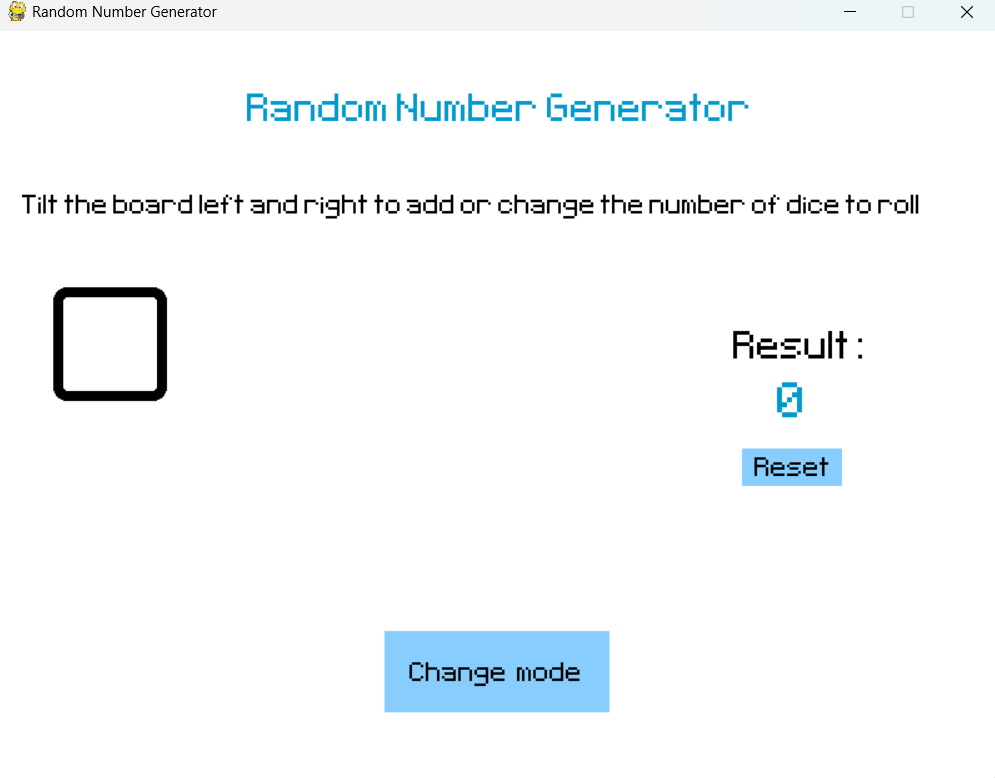
\includegraphics[width=0.7\textwidth]{HomePage.png}}
    \caption{Schermata iniziale}
    \label{fig:homepage}
\end{figure}
\\\\La visualizzazione grafica cambia in base allo stato dell'applicazione, in continuo aggiornamento in base all'interazione dell'utente.
\\In particolare, all'avvio il sistema sincronizzerà lo stato iniziale della scheda con il client, lo stato di scelta del numero di dadi.
In questo stato sarà possibile, così come da descrizione testuale, inclinare la scheda verso destra o verso sinistra per rispettivamente
incrementare o decrementare il numero di dadi. 
\\(NOTA: La velocità di risposta del client dipende dalla velocità di comunicazione 
impostata dal protocollo di comunicazione LoRa).
\\\\Interfaccia grafica nello \textbf{stato di scelta dei dadi}:
\begin{figure}[H]
    \centering
    \fbox{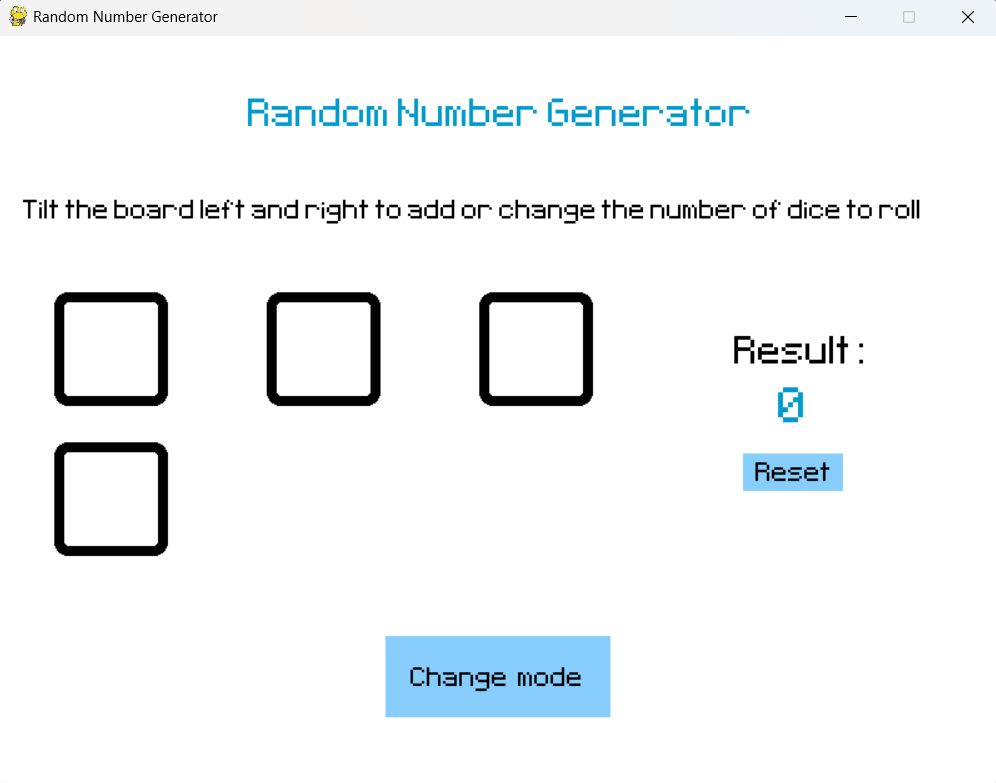
\includegraphics[width=0.7\textwidth]{RollState_OFF.png}}
    \caption{Schermata principale con 4 dadi selezionati}
    \label{fig:RollStateOFF}
\end{figure}
Il secondo stato assumibile dal sistema è quello di lancio dei dadi, in cui la descrizione testuale indica l'operazione da effettuare per 
ottenere il risultato randomico. Sarà quindi un movimento della scheda sufficientemente deciso che determinerà il valore di ciascun dado selezionato
e la conseguente visualizzazione del risultato.
\\\\Interfaccia grafica nello \textbf{stato di lancio dei dadi}:
\begin{figure}[h!]
    \centering
    \fbox{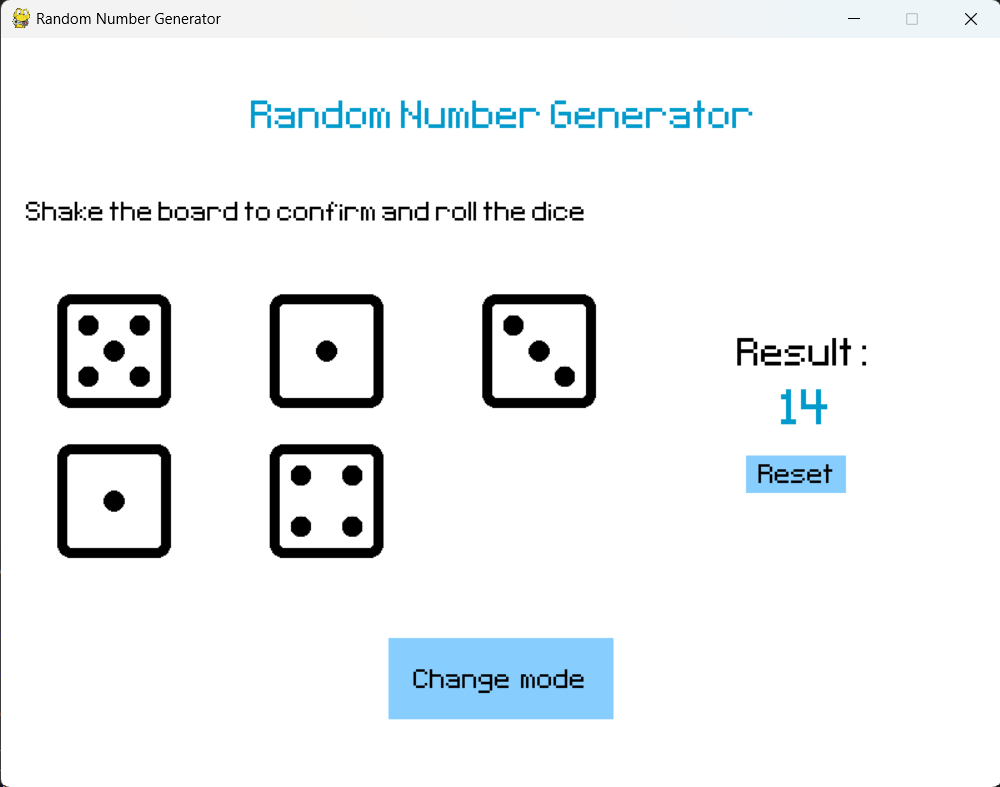
\includegraphics[width=0.7\textwidth]{RollState_ON.png}}
    \caption{Schermata principale in seguito al lancio dei dadi}
    \label{fig:RollStateON}
\end{figure}
\\Nell'interfaccia grafica ci sono due bottoni con cui è possibile interagire:
\begin{itemize}
    \item "Change mode" button, cambia lo stato del sistema
    \item "Reset" button, resetta il client e lo riporta alla schermata iniziale
\end{itemize}
\begin{figure}[h!]
    \centering
    \fbox{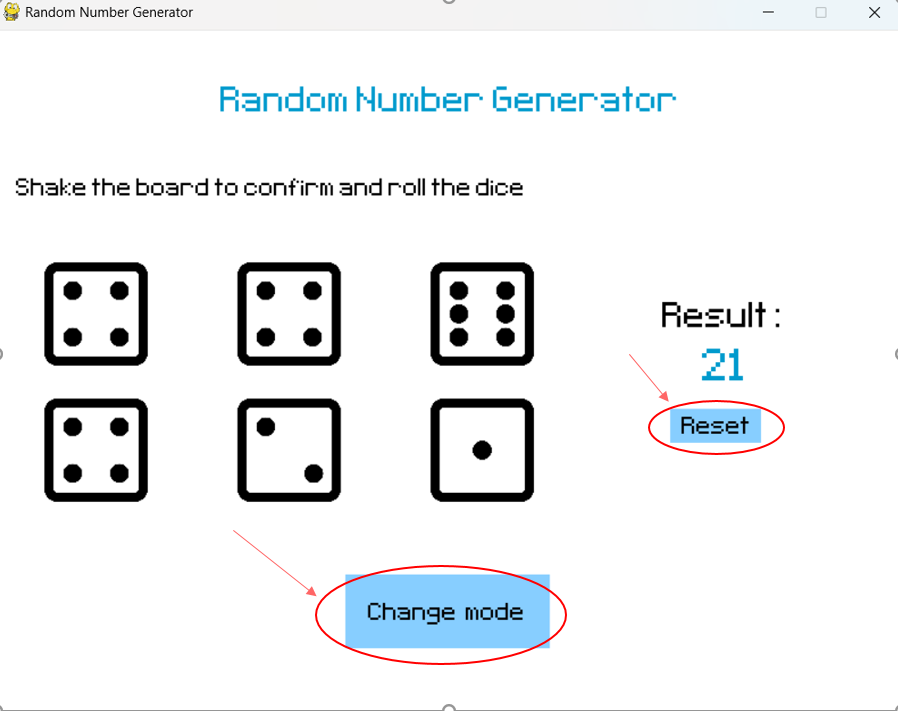
\includegraphics[width=0.7\textwidth]{HomePageButtons.png}}
    \caption{Bottoni nella schermata principale}
    \label{fig:HomePageButtons}
\end{figure}

La console del programma client python permette di visualizzare in tempo reale eventuali cambiamenti di stato dovuti alla pressione del bottone apposito, 
mostrando il payload inviato al cloud e i dettagli della comunicazione downlink tra il client, il cloud e il microcontrollore.

\begin{verbatim}
{'downlinks': [{'f_port': 2, 'priority': 'NORMAL', 'frm_payload': 'AA=='}]}

topic:
    v3/rev-gallo-application@ttn/devices/eui.......
payload:
    ...
\end{verbatim}

Analogamente, la console mostra la corretta ricezione del payload inviato dal uC al client, ad ogni nuova notifica di comunicazione uplink, 
mostrando a video i dati che permettono l'elaborazione vera e propria da parte del programma, formattati in modo leggibile.\\

È possibile consultare lo stato del sistema anche direttamente sulla scheda. Se il LED contrassegnato con il numero 3 sulla scheda principale 
è acceso significa che il sistema è nello stato di selezione del numero di dati, se spento lo stato sarà quello del lancio dei dadi.












